\documentclass{szzclass}

\usepackage{amsmath}
\usepackage{graphics}
\usepackage[export]{adjustbox}[2011/08/13]

\topic{Analytický doménový model tříd a popis životního cyklu identifikovaných tříd (cíle, UML diagram tříd, UML stavový diagram).}
\renewcommand*\contentsname{Obsah}
\author{Jakub Rathouský}
\code{BI-SPOL-06}
\subject{SI1.2}

\begin{document}
% \maketitle
\tableofcontents
\newpage

\section{Analytický doménový model tříd}
\subsection{Cíle}
\begin{itemize}
    \item popsat data
    \item popsat význam termínů
    \item popsat vazby mezi entitami
    \item identifikovat stav entity
    \item základ pro design (db model, model tříd)
    \item zachycení atributů
\end{itemize}

\section{Popis životního cyklu identifikovaných tříd (cíle, UML diagram tříd, UML stavový diagram)}
\subsection{Doménový model}
\begin{itemize}
    \item pomocí diagramu tříd UML
    \item patří do skupiny diagramů struktur
    \item využití:
    \begin{itemize}
        \item business doménový model
        \item analytický doménový model
        \item databázový model
        \item návrh modelu tříd
    \end{itemize}
    \item třída v diagramu se skládá z:
    \begin{itemize}
        \item atributů
        \item metodami
        \item viditelnost
    \end{itemize}
    \item typy vztahů:
    \begin{itemize}
        \item asociace
        \begin{itemize}
            \item udržení vztahu mezi dvěmi entitami
            \item ty mohou existovat nezávisle na sobě
            \item výchozí směr na obě strany
            \item lze přidat šipky pro upřesnění
        \end{itemize}
        \item kompozice
        \begin{itemize}
            \item podobná jako agregace, akorát silnější
            \item entita části nemá smysl bez celku
        \end{itemize}
        \item agregace - raději nepoužívat
        \begin{itemize}
            \item reprezentuje vztah celek - část
            \item celek si drží kolekci objektů
            \item část může existovat samostatně a nebo ve více kolekcích
        \end{itemize}
        \item generalization / dědičnost
    \end{itemize}
    \item násobnosti
    \begin{itemize}
        \item 0-* \dots *
        \item 1-* \dots *
        \item 0-* \dots 1
        \item \dots
    \end{itemize}
    \item popis vztahů
\end{itemize}
\begin{figure}[h!]
    \centering
    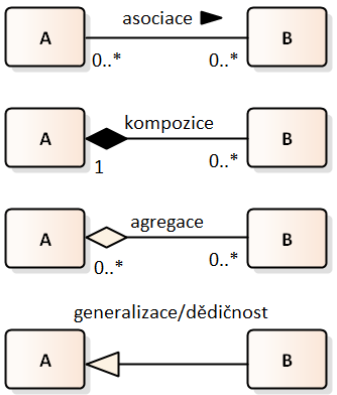
\includegraphics[width=0.6\textwidth]{topics/bi-spol-31/images/connectionTypes.png}
    \caption{Typy vztahů mezi třídami}
\end{figure}
\subsection{Atribut vs Vazba}
\begin{itemize}
    \item význam shodný
    \item důležitá je čitelnost
    \item vazba je názornější
\end{itemize}

\subsection{Hledání tříd}
\begin{itemize}
    \item předměty, objekty reálného světa
    \item podstatná jména z vytvořených dokumentů
    \begin{itemize}
        \item business model
        \item UC model
        \item slovníček pojmů
    \end{itemize}
    \item rozpracování business doménového modelu
\end{itemize}
\subsection{Cíle}
\begin{itemize}
    \item porozumět životnímu cyklu entit
    \item vyjasnění stavů, ve kterých se může entita nacházet
    \item zachyzení událostí vyvolávajících přechod a podmínek, za kterých může změna nastat
\end{itemize}

\subsection{Notace}
\begin{itemize}
    \item stavový diagram
    \begin{itemize}
        \item patří do skupiny diagramů chování
        \item konečné stavové automaty
    \end{itemize}
    \item skládá se z:
    \begin{itemize}
        \item stav
        \item přechody - události
    \end{itemize}
\end{itemize}
\begin{figure}[h!]
    \centering
    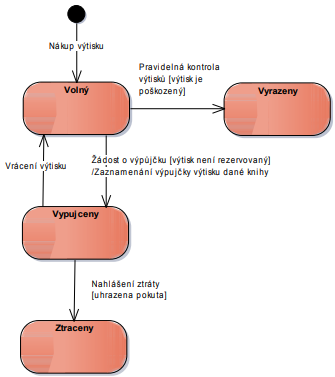
\includegraphics[width=0.6\textwidth]{topics/bi-spol-31/images/entityState.png}
    \caption{Stavový diagram}
\end{figure}
\end{document}
